%definira klasu dokumenta 
\documentclass[12pt]{report} 

%prostor izmedu naredbi \documentclass i \begin{document} se zove uvod. U njemu se nalaze naredbe koje se odnose na cijeli dokument

%osnovni LaTex ne može riješiti sve probleme, pa se koriste različiti paketi koji olakšavaju izradu željenog dokumenta
\usepackage[croatian]{babel} 
\usepackage{amssymb}
\usepackage{amsmath}
\usepackage{txfonts}
\usepackage{mathdots}
\usepackage{titlesec}
\usepackage{array}
\usepackage{lastpage}
\usepackage{etoolbox}
\usepackage{longtable, tabu}
\usepackage{color, colortbl}
\usepackage{adjustbox}
\usepackage{geometry}
\usepackage[classicReIm]{kpfonts}
\usepackage{hyperref}
\usepackage{fancyhdr}

\usepackage{float}
\usepackage{setspace}
\restylefloat{table}
\usepackage{graphicx}
\graphicspath{ {./slike/} }
\usepackage[dvipsnames]{xcolor}


\patchcmd{\chapter}{\thispagestyle{plain}}{\thispagestyle{fancy}}{}{} %redefiniranje stila stranice u paketu fancyhdr

%oblik naslova poglavlja
\titleformat{\chapter}{\normalfont\huge\bfseries}{\thechapter.}{20pt}{\Huge}
\titlespacing{\chapter}{0pt}{0pt}{40pt}


\linespread{1.3} %razmak između redaka

\geometry{a4paper, left=1in, top=1in,}  %oblik stranice

\hypersetup{ colorlinks, citecolor=black, filecolor=black, linkcolor=black,	urlcolor=black }   %izgled poveznice


%prored smanjen između redaka u nabrajanjima i popisima
\newenvironment{packed_enum}{
	\begin{enumerate}
		\setlength{\itemsep}{0pt}
		\setlength{\parskip}{0pt}
		\setlength{\parsep}{0pt}
	}{\end{enumerate}}

\newenvironment{packed_item}{
	\begin{itemize}
		\setlength{\itemsep}{0pt}
		\setlength{\parskip}{0pt}
		\setlength{\parsep}{0pt}
	}{\end{itemize}}


%boja za privatni i udaljeni kljuc u tablicama
\definecolor{LightBlue}{HTML}{1A67CB}
\definecolor{LightGreen}{HTML}{47C256}


%podesavanje zaglavlja i podnožja

\pagestyle{fancy}
\lhead{Programsko inženjerstvo}
\rhead{Najam vozila}
\lfoot{HALIKARNAS}
\cfoot{stranica \thepage/\pageref{LastPage}}
\rfoot{\today}
\renewcommand{\headrulewidth}{0.2pt}
\renewcommand{\footrulewidth}{0.2pt}


\begin{document} 
	
	
	
	\begin{titlepage}
		\begin{center}
			\vspace*{\stretch{1.0}} %u kombinaciji s ostalim \vspace naredbama definira razmak između redaka teksta
			\LARGE Programsko inženjerstvo\\
			\large Ak. god. 2020./2021.\\
			
			\vspace*{\stretch{3.0}}
			
			\huge Najam vozila\\			\Large Dokumentacija, Rev. \textit{1.0}\\
			
			\vspace*{\stretch{12.0}}
			\normalsize
			Grupa: \textit{HALIKARNAS}\\
			Voditelj: \textit{Hrvatić Josip}\\
			
			
			\vspace*{\stretch{1.0}}
			Datum predaje: \textit{13. studenog 2020.}\\
	
			\vspace*{\stretch{4.0}}
			
			Nastavnik: \textit{Miljenko Krhen}\\
		
		\end{center}

	
	\end{titlepage}

	
	\tableofcontents

	\chapter{Dnevnik promjena dokumentacije}
		
		\textbf{\textit{Kontinuirano osvježavanje}}\\
				
		
		\begin{longtabu} to \textwidth {|X[2, l]|X[13, l]|X[3, l]|X[3, l]|}
			\hline \multicolumn{1}{|l|}{\textbf{Rev.}}	& \multicolumn{1}{l|}{\textbf{Opis promjene/dodatka}} & \multicolumn{1}{|l|}{\textbf{Autori}} & \multicolumn{1}{l|}{\textbf{Datum}} \\[3pt] \hline
			\endfirsthead
			
			\hline \multicolumn{1}{|l|}{\textbf{Rev.}}	& \multicolumn{1}{l|}{\textbf{Opis promjene/dodatka}} & \multicolumn{1}{|l|}{\textbf{Autori}} & \multicolumn{1}{l|}{\textbf{Datum}} \\[3pt] \hline
			\endhead
			
			\hline 
			\endlastfoot
			
			0.1 & Napravljen predložak dokumentacije.	& Hrvatić & 28.10.2020. 		\\[3pt] \hline 
			
			0.2 & Definirani funkcionalni i nefunkcionalni zahtjevi & Ratko Sekula& 29.10.2020.\\[3pt] \hline
			
			0.3 & Definirani obrasci uporabe &Damjanović & 30.10.2020.\\[3pt] \hline
			
			0.31 & Ispravke grešaka u obrascima uporabe &Damjanović & 3.11.2020.\\[3pt] \hline
			
			0.4 & Definiran dijagram obrasca uporabe 1/3 &Blaić & 3.11.2020.\\[3pt] \hline
			
			0.41 & Definiran dijagram obrasca uporabe 2/3 &Sekula & 4.11.2020.\\[3pt] \hline
			
			0.42 & Definiran dijagram obrasca uporabe 3/3 &Smolić - Ročak & 4.11.2020.\\[3pt] \hline
			
			0.5 & Definiran sekvencijski dijagram 1/3 &Sekula & 4.11.2020.\\[3pt] \hline
			
			0.51 & Definiran sekvencijski dijagram 2/3 &Smolić - Ročak & 6.11.2020.\\[3pt] \hline
			
			0.52 & Definiran sekvencijski dijagram 3/3 &Blaić & 7.11.2020.\\[3pt] \hline

			0.6 & Dodan opis projektnog zadatka &Huđin & 10.11.2020. \\[3pt] \hline
			
			0.7 & Dodane tablice i pripadni opisi 3/6 &Blaić & 11.11.2020. \\[3pt] \hline
			
			0.8 & Dodane tablice i pripadni opisi 6/6 + ER dijagram baze podataka &Smolić - Ročak & 12.11.2020. \\[3pt] \hline
			
			0.81 & Popravak dijagrama obrasca uporabe &Sekula & 12.11.2020. \\[3pt] \hline
			
			0.82 & Dodan opis arhitekture sustava &Ratko & 13.11.2020.\\[3pt] \hline
			0.83 & Dodane fotografije u opis zadatka projekta &Huđin & 13.11.2020.\\[3pt] \hline
			0.84 & Ispravci i nadopune &Hrvatić & 13.11.2020.\\[3pt] \hline
			0.9 & Dodani dijagrami razreda i opisi &Damjanović, Hrvatić, Smolić-Ročak & 13.11.2020.\\[3pt] \hline
			
			
		\end{longtabu}
	
	
		\textit{Pošto se promjene naprave, potom se tablica ažurira.}
	\chapter{Opis projektnog zadatka}
		
		%\textbf{\textit{dio 1. revizije}}\\
		
		%\textit{Na osnovi projektnog zadatka detaljno opisati korisničke zahtjeve. Što jasnije opisati cilj projektnog zadatka, razraditi problematiku zadatka, dodati nove aspekte problema i potencijalnih rješenja. Očekuje se minimalno 3, a poželjno 4-5 stranica opisa.	Teme koje treba dodatno razraditi u ovom poglavlju su:}
		%\begin{packed_item}
			%\item \textit{potencijalna korist ovog projekta}
			%\item \textit{postojeća slična rješenja (istražiti i ukratko opisati razlike u odnosu na zadani zadatak). Dodajte slike koja predočavaju slična rješenja.} %dodaj slike %
			%\item \textit{skup korisnika koji bi mogao biti zainteresiran za ostvareno rješenje.}
			%\item \textit{mogućnost prilagodbe rješenja } 
			%\item \textit{opseg projektnog zadatka}
			%\item \textit{moguće nadogradnje projektnog zadatka}
		%\end{packed_item}
		
		%\textit{Za pomoć pogledati reference navedene u poglavlju „Popis literature“, a po potrebi konzultirati sadržaj na internetu koji nudi dobre smjernice u tom pogledu.}
		 \text Naš cilj je napraviti web aplikaciju "Autos" za iznajmljivanje vozila privatnim i poslovnim korisnicima. \par 
		 \text Cilj projekta je upoznavanje te praktična primijena postupaka oblikovanja programske podrške sa ciljem ostvarenja zahtjeva ovog zadatka, shvaćanje važnosti i značenja projektne dokumentacije te stvaranje iste. Također, od važnosti je i što preciznija implementacija zahtjeva i poboljšanje u svim područjima potrebnim za uspješno implementiranje zadatka. Uz standardno programiranje i rad dokumentacije, jedna od važnijih vještina koje ćemo dobiti je znanje o raspodjeli rada i iskustvo suradnje sa timom ljudi s ciljem ostvarenja zahtjeva. \par 
		 \text U poslovanju vezanim za iznajmljivanje automobila već postoji znatan broj tvrtki koje nude vrlo sličan model onom koji mi ostvarujemo. Priložen je jedan primjer.\par  
		 %(tu treba slika) \par 
		 \text Kao što vidimo u primjeru se nudi datum i vrijeme preuzimanja i vraćanja vozila te lokacija preuzimanja i vraćanja auta. Također se na stranicu moguće prijaviti i odabrati način plaćanja. \par 
		%\text (tu još jedna slika)
		 \text U ovom je primjeru vidljiv i izbor pojedinog automobila za iznajmljivanje. \par 
		 \text Godišnje oko 580 milijuna ljudi u svijetu koristi usluge iznajmljivanja\par  automobila, a od toga čak 70 je posto online. Ukupan broj korisnika ovih usluga kao i postotak online korištenja je u porastu te se nastavak tog porasta očekuje kroz sljedećih nekoliko godina. 
		 \text Jedan od zahtjeva ovog zadatka je stvoriti mogućnost prijave te registracije korisnika za koju je potrebno ime, prezime,  naziv institucije ili poduzeća (za službene korisnike), adresa (ulica, kućni broj,
grad, država) i adresa elektroničke pošte. \par 
         \text Implementacija će sadržavati četiri različite vrste korisnika: administrator, vlasnik sustava,\par 
korisnik (najmoprimac vozila) i neprijavljeni korisnik (gost).
        \text Administrator upisuje sve podatke o poduzeću (kao što su nove poslovnice) i definira tko ima ulogu vlasnika. Može vidjeti koliko je trenutno aktivnih korisnika i njihova imena.\par 
\text Vlasnik upisuje sve ostale potrebne podatke o vozilima, uključujući njihove tehničke
karakteristike te slike koje su prikazane na web stranici. Samo su toj ulozi 
dostupni podaci o nabavnoj cijeni vozila, troškovima održavanja i svim ostalim zavisnim
i nezavisnim troškovima vezanim uz vozila, kao i VIN oznaka svakog vozila.
Vlasniku je sustava omogućeno praćenje profitabilnosti procesa
iznajmljivanja vozila, kao i financijske performanse svakog vozila zasebno. Vlasnik vidi i koja su vozila trenutno unajmljena i na koji vremenski period te slobodna vozila. \par 
\text Registrirani korisnik ima mogućnost upravljanja svojim rezervacijama, kao što su otkazivanje ili promjena mjesta povratka vozila. Korisnik uz mogućnost rezervacije može i unajmiti vozilo na određeni vremenski period te odabrati lokaciju vraćanja i preuzimanja automobila. Sustav
mu omogućuje izbor kategorije vozila, i nakon toga točan model vozila. Ukoliko postoji
više vozila istog modela, korisnik uvijek odabire samo model, a sustav mu dodjeljuje
vozilo određeno njegovim VIM brojem. \par 
\text I gost i korisnik imaju mogućnost pregleda vozila dostupnih za najam te preglede njihovih cijena. \par 
 \text Prilikom svakog iznajmljivanja vozila najmoprimcu vozila (gostu ili korisniku) se izdaje tiskana potvrda o
preuzimanju vozila na kojoj se uz osobne podatke upisuju i podaci o trenutnom stanju
prijeđenih kilometara vozila. Također se ispisuju možebitne napomene o vozilima (oštećenja ili sl.).\par 
 \text Za izvršenje zadatka nužno je napraviti i bazu podataka koja će sadržavati sve podatke o poslovnicama, korisnicima, rezervacijama i automobilima. 
 \text Brojne su moguće nadogradnje ove implementacije. Mogli bismo dodati funkcionalnosti koje bi iskorištavale korisnikovu lokaciju i uz Google Maps automatski nudile korisniku najbliže mjesto preuzimanja vozila. Iste bi mogli iskoristiti u slučaju da je vozilo izgubljeno ili ukradeno pa bismo mogli prikazivati njegovu lokaciju i pronaći ga. 
\text Nadalje, grafička analiza podataka o isplativnosti pojedinih vozila bi vlasnicima olakšala odluke vezane za popravak, zamjenu ili nabavu novog vozila. \par 
\text Korisna bi bila i mogućnost ostavljanja recenzija za pojedino vozilo, sveukupno osoblje ili web stranicu. Recenzija bi se sastojala od ocjene i kratkog opisa. Sve bi recenzije i prosjek ocjena za svaku kategoriju ocjenjivanja mogao pregledati vlasnik. \par 
\text Dobro bi došla  funkcionalnost koja mjeri porast ukupnog i aktivnog broja korisnika te bilježi korisnike koji su najčešće mušterije. Tim bi se osobama ili poduzećima omogućilo da uđu u VIP Membership program sa određenim pogodnostima vezanim za vozila i usluge (npr. osoblje odgovara na upite 24/7, last minute rezervacije i najmovi i slično).   \par  
		\eject
		
		
		
	
	\chapter{Specifikacija programske potpore}
		
	\section{Funkcionalni zahtjevi}
			
			
			

			
			\noindent \textbf{Dionici:}
			
			\begin{packed_enum}
				
				\item Poduzeće
				\item Ovlašteni distributeri ili 'leasing' kuće				
				\item Administrator baze podataka
				\item Razvojni tim
				
			\end{packed_enum}
			
			\noindent \textbf{Aktori i njihovi funkcionalni zahtjevi:}
			
			
			\begin{packed_enum}
				\item  \underbar{Gost - neprijavljeni korisnik (inicijator) ima sljedeće mogućnosti:}
				
				\begin{packed_enum}
					
					\item pregled raspoloživih vozila poduzeća
					\item pregled mjesta razmjene vozila
					\item pristup osnovnim kontaktima poduzeća
					\item izrada vlastitog korisničkog računa
					\item odabir vlasnika uz prikaz općih informacija o vlasniku
					\item prikaz recenzija i ocjena prodavača
					\item pregled vozila po kategoriji i vrsti
					\item pregled dostupnosti vozila
					
				\end{packed_enum}
				
					\item  \underbar{Korisnik - najmoprimac (inicijator) ima sljedeće mogućnosti:}
				
				\begin{packed_enum}
					
					\item promjena osobnih podataka uz naknadnu autorizaciju administratora
					\item pregled raspoloživih vozila poduzeća
					\item pregled mjesta razmjene vozila
					\item pristup osnovnim kontaktima poduzeća
					\item pregled kategorija po kategoriji i po vrsti
					\item odabir jednog od predloženih mjesta i vremena preuzimanja i isporuke vozila za unajmljivanja
					\item korištenje posebne usluge odabira vlastitog mjesta i vremena preuzimanja i isporuke za unajmljivanja
					\item uređivanje najmova
					\item brisanje vlastitog korisničkog računa
					\item pregled prethodnih najmova
					\item pisanje recenzija i dodjeljivanje ocjena
					
				\end{packed_enum}
				
					\item  \underbar{Administrator (inicijator) ima sljedeće mogućnosti:}
				
				\begin{packed_enum}
					
					\item pregled trenutno aktivnih prijavljenih korisnika
					\item pristup kontaktima pohranjenim u bazi podataka
					\item upis podataka o poduzećima
					\item autorizacija zatraženih promjena podataka računa
					\item brisanje korisničkih računa
					\item brisanje neprimjerenih recenzija
					\item određivanje vlasnika sustava
					
				\end{packed_enum}
				
					\item  \underbar{Vlasnik (inicijator) ima sljedeće mogućnosti:}
				
				\begin{packed_enum}
					
					\item pristup statistici poduzeća
					\item pregled svih vozila u voznom parku
					\item dodavanje novih vozila
					\item pristup i promjena podataka vozila
					\item dodavanje mjesta razmjene vozila
					\item brisanje mjesta razmjene vozila
					\item kategorizacija vozila
					
				\end{packed_enum}
			
				\item  \underbar{Baza podataka (sudionik) može:}
				
				\begin{packed_enum}
					
					\item pohrana podataka o vlasnicima i pripadnim vozilima
					\item pohrana podataka o korisnicima 
					
				\end{packed_enum}
			\end{packed_enum}
			
			\eject 
			
			
				
			\subsection{Obrasci uporabe}
				
				\textbf{\textit{Dio 1. revizije}}\\
					

					\noindent \underbar{\textbf{UC 1 - Registracija korisnika}}
					\begin{packed_item}
	
						\item \textbf{Glavni sudionik: }Gost
						\item  \textbf{Cilj: }Unijeti novog korisnika u sustav
						\item  \textbf{Sudionici: }Baza podataka
						\item  \textbf{Preduvjet: }-
						\item  \textbf{Opis osnovnog tijeka: }
						
						\item[] \begin{packed_enum}
							\item Gost ulazi u zaslon za registraciju
							\item Gost unosi sve potrebne podatke
							\item Gost je registriran i sada je korisnik
						\end{packed_enum}
						
						\item  \textbf{Opis mogućih odstupanja:}
						
						\item[] \begin{packed_item}
	
							\item[2.a] Uneseni podatci nisu u pravilnom formatu
							\item[] \begin{packed_enum}
								\item Aplikacija upozorava gosta i traži ga novi unos
							\end{packed_enum}
						\end{packed_item}
					\end{packed_item}
					
					\noindent \underbar{\textbf{UC 2 - Prijava korisnika}}
					\begin{packed_item}
	
						\item \textbf{Glavni sudionik: }Gost
						\item  \textbf{Cilj: }Prijaviti se u sustav
						\item  \textbf{Sudionici: }Baza podataka
						\item  \textbf{Preduvjet: }Korisnik je registriran u sustavu
						\item  \textbf{Opis osnovnog tijeka:}
						
						\item[] \begin{packed_enum}
							\item Uđi u zaslon za prijavu u sustav
							\item Unesi podatke za prijavu
						\end{packed_enum}
						
						\item  \textbf{Opis mogućih odstupanja:}
						
						\item[] \begin{packed_item}
	
							\item[2.a]  Uneseni podatci su netočni
							\item[] \begin{packed_enum}
								\item Aplikacija upozorava korisnika i traži ga novi unos i nudi mu odlazak na zaslon za registraciju
							\end{packed_enum}
						\end{packed_item}
					\end{packed_item}
					
					\noindent \underbar{\textbf{UC 3 - Pregled osobnih podataka}}
					\begin{packed_item}
	
						\item \textbf{Glavni sudionik: }Korisnik
						\item  \textbf{Cilj: }Dobiti uvid u vlastite podatke spremljene u sustavu
						\item  \textbf{Sudionici: }Baza podataka
						\item  \textbf{Preduvjet: }Korisnik je prijavljen u sustav
						\item  \textbf{Opis osnovnog tijeka:}
						
						\item[] \begin{packed_enum}
							\item Korisnik pristupa svojoj korisničkoj stranici i time ima uvid u svoje korisničke podatke
						\end{packed_enum}
						
						\item  \textbf{Opis mogućih odstupanja: }-
					\end{packed_item}
					
					\noindent \underbar{\textbf{UC 4 - Promjena osobnih podataka}}
					\begin{packed_item}
	
						\item \textbf{Glavni sudionik: }Korisnik
						\item  \textbf{Cilj: }Urediti vlastite korisničke podatke u sustavu
						\item  \textbf{Sudionici: }Baza podataka
						\item  \textbf{Preduvjet: }Korisnik je prijavljen u sustav
						\item  \textbf{Opis osnovnog tijeka:}
						
						\item[] \begin{packed_enum}
							\item Korisnik pristupa svojoj korisničkoj stranici
							\item Klikom na odgovarajući gumb otvara se sučelje u kojem korisnik ima mogućnost uređivanja podataka
						\end{packed_enum}
						
						\item  \textbf{Opis mogućih odstupanja:}
						
						\item[] \begin{packed_item}
	
							\item[2.a] Neki od unesenih podataka nije u pravilnom formatu
							\item[] \begin{packed_enum}
								\item Aplikacija upozorava korisnika i traži ga novi unos podatka
							\end{packed_enum}
						\end{packed_item}
					\end{packed_item}
					
					\noindent \underbar{\textbf{UC 5 - Pregled prijašnjih rezervacija}}
					\begin{packed_item}
	
						\item \textbf{Glavni sudionik: }Korisnik
						\item  \textbf{Cilj: }Dobiti uvid u sve prijašnje rezervacije vozila
						\item  \textbf{Sudionici: }Baza podataka
						\item  \textbf{Preduvjet: }Korisnik je prijavljen u sustav
						\item  \textbf{Opis osnovnog tijeka:}
						
						\item[] \begin{packed_enum}
							\item Korisnik pristupa svojoj korisničkoj stranici
							\item Klikom na odgovarajući gumb prikazuju se sve prijašnje korisnikove narudžbe
						\end{packed_enum}
						
						\item  \textbf{Opis mogućih odstupanja: }-
					\end{packed_item}
					
					\noindent \underbar{\textbf{UC 6 - Brisanje korisničkog računa}}
					\begin{packed_item}
	
						\item \textbf{Glavni sudionik: }Korisnik
						\item  \textbf{Cilj: }Ukloniti zapis o korisniku iz baze podataka
						\item  \textbf{Sudionici: }Baza podataka
						\item  \textbf{Preduvjet: }Korisnik je prijavljen u sustav
						\item  \textbf{Opis osnovnog tijeka:}
						
						\item[] \begin{packed_enum}
							\item Korisnik pristupa svojoj korisničkoj stranici
							\item Prilikom uređivanja računa ima priliku i izbrisati svoj račun
							\item Klikom na odgovarajuće dugme i potvrdom odabira briše se korisnički račun
						\end{packed_enum}
						
						\item  \textbf{Opis mogućih odstupanja: }-
					\end{packed_item}
					
					\noindent \underbar{\textbf{UC 7 - Pretraga vozila}}
					\begin{packed_item}
	
						\item \textbf{Glavni sudionik: }Gost, korisnik
						\item  \textbf{Cilj: }Pretražiti slobodna vozila po određenom kriteriju
						\item  \textbf{Sudionici: }Baza podataka
						\item  \textbf{Preduvjet: }-
						\item  \textbf{Opis osnovnog tijeka:}
						
						\item[] \begin{packed_enum}
							\item Korisnik bira datum i mjesto preuzimanja te vraćanja vozila. Za to su mu na raspolaganju kalendar i popis mogućih lokacija te karta
							\item Korisnik bira kategoriju vozila koje želi unajmiti
							\item Ispisuje se popis svih vozila koje odgovaraju korisnikovim kriterijima
							\item Klikom na za to predviđeno dugme traži se rezervacija vozila
						\end{packed_enum}
						
						\item  \textbf{Opis mogućih odstupanja: }
						
						\item[] \begin{packed_item}
	                        
	                        \item[1.a] Korisnik je odabrao vrijeme izvan besplatnog perioda (9.00 - 15.00)
							\item[] \begin{packed_enum}
								\item Za to korisnik plaća dodatnu naknadu
							\end{packed_enum}
							\item[1.b] Korisnik je izabrao mjesto drukčije od onog ponuđenog u popisu predefiniranih lokacija.
							\item[] \begin{packed_enum}
								\item Za to korisnik plaća dodatnu naknadu
							\end{packed_enum}
							\item[4.a] Gost nije prijavljen u sustav i traži rezervaciju
							\item[] \begin{packed_enum}
								\item Aplikacija ga preusmjerava na zaslon za prijavu i nakon prijave mu omogućuje rezervaciju
							\end{packed_enum}
						\end{packed_item}
						
					\end{packed_item}
					
					\noindent \underbar{\textbf{UC 8 - Rezervacija vozila}}
					\begin{packed_item}
	
						\item \textbf{Glavni sudionik: }Korisnik
						\item  \textbf{Cilj: }Rezervirati vozilo za iznajmljivanje
						\item  \textbf{Sudionici: }Baze podataka
						\item  \textbf{Preduvjet: }Korisnik je prijavljen u sustav i postoje slobodna vozila
						\item  \textbf{Opis osnovnog tijeka:}
						
						\item[] \begin{packed_enum}
							\item Korisnik pretražuje vozilo po prethodnom scenariju
							\item Klikom na željeno vozilo otvara se zaslon za plaćanje, na kojem korisnik plaća za rezervaciju zajedno s predujmom
							\item Rezervacija je napravljena i vidljiva je na korisničkim stranicama
						\end{packed_enum}
						
						\item  \textbf{Opis mogućih odstupanja: }-
					\end{packed_item}
					
					\noindent \underbar{\textbf{UC 9 - Promjena rezervacije}}
					\begin{packed_item}
	
						\item \textbf{Glavni sudionik: }Korisnik
						\item  \textbf{Cilj: }Urediti postojeću rezervaciju produljivanjem ili skraćivanjem perioda rezervacije
						\item  \textbf{Sudionici: }Baza podataka
						\item  \textbf{Preduvjet: }Postoji aktivna rezervacija i vozilo mora biti dostupno u novom željenom terminu
						\item  \textbf{Opis osnovnog tijeka:}
						
						\item[] \begin{packed_enum}
							\item Korisnik odlazi na popis svojih rezervacija.
							\item Klikom na odgovarajući gum ima opciju promijeniti datum preuzimanja (ako vozilo već nije preuzeto) i vraćanja vozila.
							\item Dodatni iznos za plaćanje koji je nastao razriješit će se prilikom povrata vozila.
						\end{packed_enum}
						
						\item  \textbf{Opis mogućih odstupanja: }
						
						\item[] \begin{packed_item}
	
							\item[2.a] Vozilo u novoodabranom terminu nije dostupno
							\item[] \begin{packed_enum}
								\item Aplikacija upozorava korisnika i ne dozvoljava mu postavljanje na taj datum.
							\end{packed_enum}
						\end{packed_item}
					\end{packed_item}
					
					\noindent \underbar{\textbf{UC 10 - Otkazivanje rezervacije}}
					\begin{packed_item}
	
						\item \textbf{Glavni sudionik: }Korisnik
						\item  \textbf{Cilj: }Otkazati napravljenu rezervaciju
						\item  \textbf{Sudionici: }Baza podataka
						\item  \textbf{Preduvjet: }Korisnik je prijavljen u sustav i postoji aktivna rezervacija, a vozilo još nije preuzeto
						\item  \textbf{Opis osnovnog tijeka:}
						
						\item[] \begin{packed_enum}
							\item Korisnik odlazi na popis aktivnih rezervacija.
							\item Iz popisa bira aktivnu rezervaciju koju želi otkazati
							\item Klikom na odgovarajući gumn korisnik briše rezervaciju
						\end{packed_enum}
						
						\item  \textbf{Opis mogućih odstupanja: }
						
						\item[] \begin{packed_item}
	
							\item[3.a] Do predviđenog vremena preuzimanja ostala su manje od 24 sata 
							\item[] \begin{packed_enum}
								\item Korisniku se naplaćuje određen iznos
							\end{packed_enum}
						\end{packed_item}
					\end{packed_item}
					
					\noindent \underbar{\textbf{UC 11 - Recenziranje usluge}}
					\begin{packed_item}
	
						\item \textbf{Glavni sudionik: }Korisnik
						\item  \textbf{Cilj: }Nakon povrata bozila ostaviti recenziju na uslugu
						\item  \textbf{Sudionici: }Baza podataka
						\item  \textbf{Preduvjet: }Korisnik je prijavljen, a usluga koja se ocjenjuje završila je
						\item  \textbf{Opis osnovnog tijeka:}
						
						\item[] \begin{packed_enum}
							\item Korisnik u popisu svojih prijašnjih rezervacija može recenzirati i mijenjati postojeće recenzije u rangu od jedne do pet zvjezdica
						\end{packed_enum}
						
						\item  \textbf{Opis mogućih odstupanja: }-
					\end{packed_item}
					
					\noindent \underbar{\textbf{UC 12 - Prikaz karte s navedenim poslovnicama}}
					\begin{packed_item}
	
						\item \textbf{Glavni sudionik: }Gost, korisnik, vlasnik sustava
						\item  \textbf{Cilj: }Na karti vidjeti prikazane sve poslovnice tvtrke za rent-a-car
						\item  \textbf{Sudionici: }Baza podataka
						\item  \textbf{Preduvjet: }-
						\item  \textbf{Opis osnovnog tijeka:}
						
						\item[] \begin{packed_enum}
							\item Prikaz karte bit će dostupan na naslovnoj stranici aplikacije te prilikom odabira mjesta preuzimanja i povrata vozila
							\item Na karti će biti označene poslovnice na koje će se moći kliknuti i vidjeti informacije o toj poslovnici, ili ju odabrati kao lokaciju preuzimanja i/ili povrata vozila
						\end{packed_enum}
						
						\item  \textbf{Opis mogućih odstupanja: }-
					\end{packed_item}
					
					\noindent \underbar{\textbf{UC 13 - Dodavanje vozila}}
					\begin{packed_item}
	
						\item \textbf{Glavni sudionik: }Vlasnik sustava
						\item  \textbf{Cilj: }Dodati novo vozilo u bazu podataka
						\item  \textbf{Sudionici: }Baza podataka
						\item  \textbf{Preduvjet: }Vlasnik je prijavljen u usustav
						\item  \textbf{Opis osnovnog tijeka:}
						
						\item[] \begin{packed_enum}
							\item U sučelju određenom za uređivanje popisa vozila vlasnik ima opciju dodavanja novog vozila
							\item Vlasnik unosi sve potrebne informacije o vozilu; slike, tehničke specifikacije, kategoriju i slično.
							\item Vozilo je sada vidljivo korisnicima i spremno za iznajmljivanje
						\end{packed_enum}
						
						\item  \textbf{Opis mogućih odstupanja: }
						
						\item[] \begin{packed_item}
	
							\item[2.a] Neki od unesenih podataka nisu u pravilnom formatu
							\item[] \begin{packed_enum}
								\item Aplikacija upozorava vlasnika i traži ga točan unos
							\end{packed_enum}
						\end{packed_item}
					\end{packed_item}
					
					\noindent \underbar{\textbf{UC 14 - Uklanjanje vozila}}
					\begin{packed_item}
	
						\item \textbf{Glavni sudionik: }Vlasnik sustava
						\item  \textbf{Cilj: }Neko vozilo ukloniti iz baze podataka
						\item  \textbf{Sudionici: }Baza podataka
						\item  \textbf{Preduvjet: }Vlasnik je prijavljen u usustav
						\item  \textbf{Opis osnovnog tijeka:}
						
						\item[] \begin{packed_enum}
							\item U sučelju određenom za uređivanje popisa vozila vlasnik ima opciju uklanjanja vozila
							\item Klikom na za to predviđeno digme i potvrdom vozilo će se ukloniti iz baze
							\item Vozilo više nije vidljivo korisnicima i ne može se unajmiti. 
						\end{packed_enum}
						
						\item  \textbf{Opis mogućih odstupanja: }-
					\end{packed_item}
					
					\noindent \underbar{\textbf{UC 15 - Uređivanje podataka o vozilu}}
					\begin{packed_item}
	
						\item \textbf{Glavni sudionik: }Vlasnik sustava
						\item  \textbf{Cilj: }Urediti određene informacije o vozilu
						\item  \textbf{Sudionici: }Baza podataka
						\item  \textbf{Preduvjet: }Vlasnik je prijavljen u usustav
						\item  \textbf{Opis osnovnog tijeka:}
						
						\item[] \begin{packed_enum}
							\item U sučelju određenom za uređivanje popisa vozila vlasnik ima opciju uređivanja informacija o vozilu
							\item Vlasnik mijenja podatke o vozilu
							\item Promjene su sada vidljive korisnicima 
						\end{packed_enum}
						
						\item  \textbf{Opis mogućih odstupanja: }
						
						\item[] \begin{packed_item}
	
							\item[2.a] Neki od unesenih podataka nisu u pravilnom formatu
							\item[] \begin{packed_enum}
								\item Aplikacija upozorava vlasnika i traži ga točan unos
							\end{packed_enum}
						\end{packed_item}
					\end{packed_item}
					
					\noindent \underbar{\textbf{UC 16 - Prikaz profitabilnosti i prijašnjih narudžbi}}
					\begin{packed_item}
	
						\item \textbf{Glavni sudionik: }Vlasnik sustava
						\item  \textbf{Cilj: }Dobiti uvid u sve prijašnje narudžbe i prikaz profitabilnosti procesa
						\item  \textbf{Sudionici: }Baza podataka
						\item  \textbf{Preduvjet: }Vlasnik je prijavljen u sustav
						\item  \textbf{Opis osnovnog tijeka:}
						
						\item[] \begin{packed_enum}
							\item U sučelju određenom za praćenje narudžbi vlasnik ima opciju pregledati povijest svih dosadašnjih narudžbi
							\item Vlasnik bira za koji vremenski period želi pregledati narudžbe, npr. all-time, prošlu godinu, prošli mjesec, prosinac 2018. i slično.
							\item Povijest se prikazuje u obliku popisa ili grafički, ovisno kako to korisnik odabere
						\end{packed_enum}
						
						\item  \textbf{Opis mogućih odstupanja:}
						
						\item[] \begin{packed_item}
	
							\item[2.a] Ne postoje narudžbe u odabranom vremenskom periodu
							\item[] \begin{packed_enum}
								\item Umjesto popisa se ispisuje prikladna poruka
							\end{packed_enum}
						\end{packed_item}
					\end{packed_item}
					
					\noindent \underbar{\textbf{UC 17 - Prikaz slobodnih vozila}}
					\begin{packed_item}
	
						\item \textbf{Glavni sudionik: }Vlasnik sustava
						\item  \textbf{Cilj: }Dobiti uvid u popis trenutno slobodnih vozila
						\item  \textbf{Sudionici: }Baza podataka
						\item  \textbf{Preduvjet: }Vlasnik je prijavljen u sustav
						\item  \textbf{Opis osnovnog tijeka:}
						
						\item[] \begin{packed_enum}
							\item U sučelju određenom za praćenje narudžbi vlasnik ima opciju pregledati sva trenutno slobodna vozila
						\end{packed_enum}
						
						\item  \textbf{Opis mogućih odstupanja:}
						
						\item[] \begin{packed_item}
	
							\item[1.a] Ne postoje slobodna vozila
							\item[] \begin{packed_enum}
								\item Umjesto popisa se ispisuje prikladna poruka
							\end{packed_enum}
						\end{packed_item}
					\end{packed_item}
					
					\noindent \underbar{\textbf{UC 18 - Prikaz aktivnih rezervacija}}
					\begin{packed_item}
	
						\item \textbf{Glavni sudionik: }Vlasnik sustava
						\item  \textbf{Cilj: }Dobiti uvid u popis trenutno zauzetih vozila
						\item  \textbf{Sudionici: }Baza podataka
						\item  \textbf{Preduvjet: }Vlasnik je prijavljen u sustav
						\item  \textbf{Opis osnovnog tijeka:}
						
						\item[] \begin{packed_enum}
							\item U sučelju određenom za praćenje narudžbi vlasnik ima opciju pregledati sva trenutno zauzeta vozila
							\item Prikazuju se osnovne info o zauzetom vozilu, npr. ime korisnika koji trenutno koristi uslugu, predviđeno vrijeme vraćanja i sl.
						\end{packed_enum}
						
						\item  \textbf{Opis mogućih odstupanja:}
						
						\item[] \begin{packed_item}
	
							\item[2.a] Ne postoje zauzeta vozila
							\item[] \begin{packed_enum}
								\item Umjesto popisa se ispisuje prikladna poruka
							\end{packed_enum}
						\end{packed_item}
					\end{packed_item}
					
					\noindent \underbar{\textbf{UC 19 - Zatvaranje rezervacije}}
					\begin{packed_item}
	
						\item \textbf{Glavni sudionik: }Vlasnik vozila
						\item  \textbf{Cilj: }Rezervaciju označiti gotovom
						\item  \textbf{Sudionici: }Baza podataka
						\item  \textbf{Preduvjet: }Vlasnik je prijavljen u sustav, rezervacija je trenutno aktivna
						\item  \textbf{Opis osnovnog tijeka:}
						
						\item[] \begin{packed_enum}
							\item Po povratu vozila vlasnik sustava vrši pregled vozila kako bi se utvrdila možebitna oštećenja na vozilu
							\item Vlasnik izdaje pisanu potvrdu o završetku rezervacije i korisnik i vlasnik se novčano razdužuju
							\item Vlasnik rezervaciju označava završenom i vozilo je ponovo dostupno za iznajmljivanje drugim korisnicima
							\item Narudžba je sada vidljiva u popisu prošlih narudžbi
							\item Korisnik potvrdu vidi u svojim prijašnjim narudžbama
						\end{packed_enum}
						
						\item  \textbf{Opis mogućih odstupanja:} -
					\end{packed_item}
					
					
					\noindent \underbar{\textbf{UC 20 - Pregled korisnika}}
					\begin{packed_item}
	
						\item \textbf{Glavni sudionik: }Administrator
						\item  \textbf{Cilj: }Dobiti uvid u popis korisnika u bazi
						\item  \textbf{Sudionici: }Baza podataka
						\item  \textbf{Preduvjet: }Korisnik ima administratrorska prava
						\item  \textbf{Opis osnovnog tijeka:}
						
						\item[] \begin{packed_enum}
							\item Administrator ima uvid u popis svih korisnika prijavljenih u bazu
							\item Klikom na određenog korisnika iz popisa administrator ima uvid u sve podatke o njemu koji su u bazi zapisani
						\end{packed_enum}
						
						\item  \textbf{Opis mogućih odstupanja: }-
					\end{packed_item}
					
					\noindent \underbar{\textbf{UC 21 - Brisanje korisnika}}
					\begin{packed_item}
	
						\item \textbf{Glavni sudionik: }Administrator
						\item  \textbf{Cilj: }Određenog korisnika izbrisati iz baze
						\item  \textbf{Sudionici: }Baza podataka
						\item  \textbf{Preduvjet: }Korisnik ima administratorska prava
						\item  \textbf{Opis osnovnog tijeka:}
						
						\item[] \begin{packed_enum}
							\item Administrator ima uvid u popis svih korisnika prijavljenih u bazu
							\item Klikom na određenog korisnika administrator ima uvid u njega
							\item Klikom na odgovarajući gumn i potvrdom administrator briše korisnika
						\end{packed_enum}
						
						\item  \textbf{Opis mogućih odstupanja:}
						
						\item[] \begin{packed_item}
	
							\item[3.a] Administrator pokušava izbrisati samog sebe 
							\item[] \begin{packed_enum}
								\item Aplikacija mu to ne dozvoljava i javlja mu poruku
							\end{packed_enum}
						\end{packed_item}
					\end{packed_item}
					
					\noindent \underbar{\textbf{UC 22 - Promjena razine korisnika}}
					\begin{packed_item}
	
						\item \textbf{Glavni sudionik: }Administrator
						\item  \textbf{Cilj: }Za određenog korisnika promijeniti razinu prava
						\item  \textbf{Sudionici: }Baza podataka
						\item  \textbf{Preduvjet: }Korisnik ima administratorska prava
						\item  \textbf{Opis osnovnog tijeka:}
						
						\item[] \begin{packed_enum}
							\item Administrator ima uvid u popis svih korisnika prijavljenih u sustav
							\item Klikom na odrešenog korisnika administrator ima uvid u njega
							\item Administrator može promijeniti razinu korisnika, iz običnog u vlasnika sustava i obrnuto
						\end{packed_enum}
						
						\item  \textbf{Opis mogućih odstupanja:}
						
						\item[] \begin{packed_item}
	
							\item[2.a] Administrator pokušava promijeniti svoja prava iz administratorskih prava u neko niže
							\item[] \begin{packed_enum}
								\item Aplikacija mu to ne dozvoljava i javlja mu poruku
							\end{packed_enum}
						\end{packed_item}
					\end{packed_item}
					
					\noindent \underbar{\textbf{UC 23 - Dodavanje poslovnice}}
					\begin{packed_item}
	
						\item \textbf{Glavni sudionik: }Administrator
						\item  \textbf{Cilj: }Dodati novu poslovnicu u bazu podataka
						\item  \textbf{Sudionici: }Baza podataka
						\item  \textbf{Preduvjet: }Korisnik ima administratorska prava
						\item  \textbf{Opis osnovnog tijeka:}
						
						\item[] \begin{packed_enum}
							\item Administrator u sučelju ima mogućnost pregleda popisa svih poslovnica tvrtke
							\item Klikom na odgovarajuće dugme može dodati novu poslovicu
							\item Administrator dodaje sve potrebne informacije o poslovnici; Adresa, kontakt broj i sl.
							\item Ta je poslovnica vidljiva svim korisnicima u aplikaciji
						\end{packed_enum}
						
						\item  \textbf{Opis mogućih odstupanja: }
						
						\item[] \begin{packed_item}
	
							\item[3.a] Neki od unesenih podataka nisu u pravilnom formatu
							\item[] \begin{packed_enum}
								\item Aplikacija upozorava administratora i traži ga novi unos
							\end{packed_enum}
						\end{packed_item}
						
					\end{packed_item}
					
					\noindent \underbar{\textbf{UC 24 - Uklanjanje poslovnice}}
					\begin{packed_item}
	
						\item \textbf{Glavni sudionik: }Administrator
						\item  \textbf{Cilj: }Ukloniti poslovnicu iz baze podataka
						\item  \textbf{Sudionici: }Baza podataka
						\item  \textbf{Preduvjet: }Korisnik ima administratorska prava i postoje unesene poslovnice
						\item  \textbf{Opis osnovnog tijeka:}
						
						\item[] \begin{packed_enum}
							\item Administrator u sučelju ima mogućnost pregleda popisa svih poslovnica tvrtke
							\item Klikom na odgovarajuće dugme i potvrdom administrator uklanja poslovnicu
							\item Poslovnica više nije vidljiva korisnicima u aplikaciji
						\end{packed_enum}
						
						\item  \textbf{Opis mogućih odstupanja: }-
					\end{packed_item}
					
					\noindent \underbar{\textbf{UC 25 - Uređivanje poslovnice}}
					\begin{packed_item}
	
						\item \textbf{Glavni sudionik: }Administrator
						\item  \textbf{Cilj: }Urediti podatke o poslovnici
						\item  \textbf{Sudionici: }Baza podataka
						\item  \textbf{Preduvjet: }Korisnik ima administratorska prava i postoje unesene poslovnice
						\item  \textbf{Opis osnovnog tijeka:}
						
						\item[] \begin{packed_enum}
							\item Administrator u sučelju ima mogućnost pregleda popisa svih poslovnica tvrtke
							\item Klikom na određeno dugme administrator pristupa sučelju za uređivanje podataka o poslovnici
							\item Administrator unosi nove podatke i snima promjene
							\item Promjene su vidljive korisnicima u aplikaciji
						\end{packed_enum}
						
						\item  \textbf{Opis mogućih odstupanja: }
						
						\item[] \begin{packed_item}
	
							\item[3.a] Neki od unesenih podataka nisu u pravilnom formatu
							\item[] \begin{packed_enum}
								\item Aplikacija upozorava administratora i traži ga novi unos
							\end{packed_enum}
						\end{packed_item}
						
					\end{packed_item}
				
					
				\subsubsection{Dijagrami obrazaca uporabe}
					
					\textit{Prikazati odnos aktora i obrazaca uporabe odgovarajućim UML dijagramom. Nije nužno nacrtati sve na jednom dijagramu. Modelirati po razinama apstrakcije i skupovima srodnih funkcionalnosti.}
				\eject		
				
			\subsection{Sekvencijski dijagrami}
				
				\textbf{\textit{dio 1. revizije}}\\
				
				\textit{Nacrtati sekvencijske dijagrame koji modeliraju najvažnije dijelove sustava (max. 4 dijagrama). Ukoliko postoji nedoumica oko odabira, razjasniti s asistentom. Uz svaki dijagram napisati detaljni opis dijagrama.}
				\eject
	
		\section{Nefunkcionalni zahtjevi}
		
		    	\textbf{\textit{Zahtjevi kvalitete:}}\\
		 
		\begin{packed_item}
	
						\item Sustav bi trebao jamčiti točnost i pouzdanost informacija.
						\item  Unos neispravnih oblika podataka ili upload krivih datoteka ne smije narušiti sustav.
						\item Odgovor na svaki upit ili zahtjev za nekom radnjom nebi trebao trajati duže od 1 sekunde.
						\item  Dizajn sustava mora omogućiti intuitivnu uporabu sustava.
						\item Sustav se mora moći nadograditi prema zahtjevima naručitelja
						
					\end{packed_item}
				
			 
	    	\textbf{\textit{Ograničenja:}}\\
		 
			\begin{packed_item}
	
						\item Programska podrška je izvedena kao Springboot web aplikacija pisana u Javi.
						\item  Pohrana podataka je izvedena preko Postgre SQL baze podataka.
						\item Programska podrška mora bit sposobna na CRUD operacije svih priloženih podataka.
						\item  Jedan korisnik ne može biti ulogiran na dva različita računala(istovremeno imati dvije aktivne sjednice)
						
					\end{packed_item}
			 
			 
			 
	
	\chapter{Arhitektura i dizajn sustava}
		
		\textbf{\textit{dio 1. revizije}}\\

		\textit{ Potrebno je opisati stil arhitekture te identificirati: podsustave, preslikavanje na radnu platformu, spremišta podataka, mrežne protokole, globalni upravljački tok i sklopovsko-programske zahtjeve. Po točkama razraditi i popratiti odgovarajućim skicama:}
	\begin{itemize}
		\item 	\textit{izbor arhitekture temeljem principa oblikovanja pokazanih na predavanjima (objasniti zašto ste baš odabrali takvu arhitekturu)}
		\item 	\textit{organizaciju sustava s najviše razine apstrakcije (npr. klijent-poslužitelj, baza podataka, datotečni sustav, grafičko sučelje)}
		\item 	\textit{organizaciju aplikacije (npr. slojevi frontend i backend, MVC arhitektura) }		
	\end{itemize}

	
		

		

				
		\section{Baza podataka}
			
			\textbf{\textit{dio 1. revizije}}\\
			
		\textit{Potrebno je opisati koju vrstu i implementaciju baze podataka ste odabrali, glavne komponente od kojih se sastoji i slično.}
		
		    \noindent Za potrebe našeg sustava koristit ćemo relacijsku bazu podataka koja
            svojom strukturom olakšava modeliranje stvarnog svijeta. Gradivna jedinka
            baze je relacija, odnosno tablica koja je definirana svojim imenom i 
            skupom atributa. Zadaća baze podataka je brza i jednostavna pohrana, 
            izmjena i dohvat podataka za daljnju obradu.
            Baza podataka ove aplikacije sastoji se od sljedećih entiteta:
            
            \begin{packed_item}
                \item Korisnik
                \item Poslovnica
                \item Recenzija
                \item Rezervacija
                \item Session
                \item Vozilo
            \end{packed_item}
		
			\subsection{Opis tablica}
			

				\textit{Svaku tablicu je potrebno opisati po zadanom predlošku. Lijevo se nalazi točno ime varijable u bazi podataka, u sredini se nalazi tip podataka, a desno se nalazi opis varijable. Svjetlozelenom bojom označite primarni ključ. Svjetlo plavom označite strani ključ}
				
				\begin{longtabu} to \textwidth {|X[6, l]|X[6, l]|X[20, l]|}
					
					\hline \multicolumn{3}{|c|}{\textbf{korisnik - ime tablice}}	 \\[3pt] \hline
					\endfirsthead
					
					\hline \multicolumn{3}{|c|}{\textbf{korisnik - ime tablice}}	 \\[3pt] \hline
					\endhead
					
					\hline 
					\endlastfoot
					
					\cellcolor{LightGreen}IDKorisnik & INT	&  	Quo usque tandem abutere, Catilina, patientia nostra? quam diu etiam furor iste tuus nos eludet? quem ad finem sese effrenata iactabit audacia tua? Nihilne te nocturnum praesidium Palati, nihil urbis vigiliae, nihil timor populi, nihil concursus bonorum omnium, nihil hic munitissimus habendi senatus locus, nihil horum ora voltusque moverunt? 	\\ \hline
					korisnickoIme	& VARCHAR &   Patere tua consilia non sentis, constrictam iam horum omnium scientia teneri coniurationem tuam non vides? Quid proxima, quid superiore nocte egeris, ubi fueris, quos convocaveris, quid consilii ceperis, quem nostrum ignorare arbitraris?\\ \hline 
					email & VARCHAR &   \\ \hline 
					ime & VARCHAR	&  		\\ \hline 
					\cellcolor{LightBlue} primjer	& VARCHAR &   	\\ \hline 
					
					
				\end{longtabu}
				
				\noindent \textbf{Korisnik} \quad Ovaj entitet sadržava sve važne informacije o korisniku aplikacije. Sadrži atribute: Korisničko ime, ime, prezime, email, lozinku, broj mobitela korisnika i njegovu ulogu. Ovaj entitet u vezi je
                \textit{One-to-Many} s entitetom Recenzija preko atributa korisničko ime korisnika i u vezi \textit{One-to-Many} s entitetom Rezervacija preko korisničkog imena.
                
                \begin{longtabu} to \textwidth {|X[6, l]|X[6, l]|X[20, l]|}
					
					\hline \multicolumn{3}{|c|}{\textbf{Korisnik}}	 \\[3pt] \hline
					\endfirsthead
					
					\hline \multicolumn{3}{|c|}{\textbf{Korisnik}}	 \\[3pt] \hline
					\endhead
					
					\hline 
					\endlastfoot
					
					\cellcolor{LightGreen}Korisničko ime & VARCHAR	&  	korisničko ime korisnika koje je ujedno i jedinstveni identifikator\\ \hline
					Ime	& VARCHAR &   ime korisnika\\ \hline
					Prezime	& VARCHAR &   prezime korisnika\\ \hline
					Email & VARCHAR &   e-mail adresa korisnika\\ \hline
					Lozinka	& VARCHAR &   lozinka korisnika\\ \hline
					Broj mobitela	& VARCHAR &   broj mobitela korisnika\\ \hline 
					Uloga	& VARCHAR &   definira razinu ovlasti korisnika\\ \hline
					
					
				\end{longtabu}
				
				\noindent \textbf{Poslovnica} \quad Ovaj entitet sadržava sve važne informacije o poslovnici. Sadrži atribute: ID poslovnice i lokaciju poslovnice.
				
				\begin{longtabu} to \textwidth {|X[6, l]|X[6, l]|X[20, l]|}
					
					\hline \multicolumn{3}{|c|}{\textbf{Poslovnica}}	 \\[3pt] \hline
					\endfirsthead
					
					\hline \multicolumn{3}{|c|}{\textbf{Poslovnica}}	 \\[3pt] \hline
					\endhead
					
					\hline 
					\endlastfoot
					
					\cellcolor{LightGreen}ID poslovnice & INT	&  	jedinstveni identifikator poslovnice\\ \hline
					Lokacija	& VARCHAR &   adresa poslovnice\\ \hline
					
					
				\end{longtabu}
				
				\noindent \textbf{Recenzija} \quad Ovaj entitet sadržava sve važne informacije vezane za osvrt korisnika o pruženoj usluzi. Sadrži atribute: ID recenzije,
                ocjenu usluge, opis i korisničko ime korisnika koji ocjenjuje uslugu.
                Ovaj entitet u vezi je \textit{Many-to-One} s entitetom Korisnik preko korisničkog imena.
                
                \begin{longtabu} to \textwidth {|X[6, l]|X[6, l]|X[20, l]|}
					
					\hline \multicolumn{3}{|c|}{\textbf{Recenzija}}	 \\[3pt] \hline
					\endfirsthead
					
					\hline \multicolumn{3}{|c|}{\textbf{Recenzija}}	 \\[3pt] \hline
					\endhead
					
					\hline 
					\endlastfoot
					
					\cellcolor{LightGreen}ID recenzije & INT	&  	jedinstveni identifikator recenzije\\ \hline
					Ocjena	& INT &   ocjena za uslugu\\ \hline
					Opis	& VARCHAR &   komentar na ocjenu usluge\\ \hline
					\cellcolor{LightBlue}Korisničko ime	& VARCHAR &   jedinstveni identifikator korisnika, (korisnik.korisničko ime)	\\ \hline 
					
					
				\end{longtabu}
			
			
			\subsection{Dijagram baze podataka}
				\textit{ U ovom potpoglavlju potrebno je umetnuti dijagram baze podataka. Primarni i strani ključevi moraju biti označeni, a tablice povezane. Bazu podataka je potrebno normalizirati. Podsjetite se kolegija "Baze podataka".}
			
			\eject
			
			
		\section{Dijagram razreda}
		
			\textit{Potrebno je priložiti dijagram razreda s pripadajućim opisom. Zbog preglednosti je moguće dijagram razlomiti na više njih, ali moraju biti grupirani prema sličnim razinama apstrakcije i srodnim funkcionalnostima.}\\
			
			\textbf{\textit{dio 1. revizije}}\\
			
			\textit{Prilikom prve predaje projekta, potrebno je priložiti potpuno razrađen dijagram razreda vezan uz \textbf{generičku funkcionalnost} sustava. Ostale funkcionalnosti trebaju biti idejno razrađene u dijagramu sa sljedećim komponentama: nazivi razreda, nazivi metoda i vrste pristupa metodama (npr. javni, zaštićeni), nazivi atributa razreda, veze i odnosi između razreda.}\\
			
			\textbf{\textit{dio 2. revizije}}\\			
			
			\textit{Prilikom druge predaje projekta dijagram razreda i opisi moraju odgovarati stvarnom stanju implementacije}
			
			
			
			\eject
		
		\section{Dijagram stanja}
			
			
			\textbf{\textit{dio 2. revizije}}\\
			
			\textit{Potrebno je priložiti dijagram stanja i opisati ga. Dovoljan je jedan dijagram stanja koji prikazuje \textbf{značajan dio funkcionalnosti} sustava. Na primjer, stanja korisničkog sučelja i tijek korištenja neke ključne funkcionalnosti jesu značajan dio sustava, a registracija i prijava nisu. }
			
			
			\eject 
		
		\section{Dijagram aktivnosti}
			
			\textbf{\textit{dio 2. revizije}}\\
			
			 \textit{Potrebno je priložiti dijagram aktivnosti s pripadajućim opisom. Dijagram aktivnosti treba prikazivati značajan dio sustava.}
			
			\eject
		\section{Dijagram komponenti}
		
			\textbf{\textit{dio 2. revizije}}\\
		
			 \textit{Potrebno je priložiti dijagram komponenti s pripadajućim opisom. Dijagram komponenti treba prikazivati strukturu cijele aplikacije.}
	\chapter{Implementacija i korisničko sučelje}
		
		
		\section{Korištene tehnologije i alati}
		
			\textbf{\textit{dio 2. revizije}}
			
			 \textit{Detaljno navesti sve tehnologije i alate koji su primijenjeni pri izradi dokumentacije i aplikacije. Ukratko ih opisati, te navesti njihovo značenje i mjesto primjene. Za svaki navedeni alat i tehnologiju je potrebno \textbf{navesti internet poveznicu} gdje se mogu preuzeti ili više saznati o njima}.
			
			
			\eject 
		
	
		\section{Ispitivanje programskog rješenja}
			
			\textbf{\textit{dio 2. revizije}}\\
			
			 \textit{U ovom poglavlju je potrebno opisati provedbu ispitivanja implementiranih funkcionalnosti na razini komponenti i na razini cijelog sustava s prikazom odabranih ispitnih slučajeva. Studenti trebaju ispitati temeljnu funkcionalnost i rubne uvjete.}
	
			
			\subsection{Ispitivanje komponenti}
			\textit{Potrebno je provesti ispitivanje jedinica (engl. unit testing) nad razredima koji implementiraju temeljne funkcionalnosti. Razraditi \textbf{minimalno 6 ispitnih slučajeva} u kojima će se ispitati redovni slučajevi, rubni uvjeti te izazivanje pogreške (engl. exception throwing). Poželjno je stvoriti i ispitni slučaj koji koristi funkcionalnosti koje nisu implementirane. Potrebno je priložiti izvorni kôd svih ispitnih slučajeva te prikaz rezultata izvođenja ispita u razvojnom okruženju (prolaz/pad ispita). }
			
			
			
			\subsection{Ispitivanje sustava}
			
			 \textit{Potrebno je provesti i opisati ispitivanje sustava koristeći radni okvir Selenium\footnote{\url{https://www.seleniumhq.org/}}. Razraditi \textbf{minimalno 4 ispitna slučaja} u kojima će se ispitati redovni slučajevi, rubni uvjeti te poziv funkcionalnosti koja nije implementirana/izaziva pogrešku kako bi se vidjelo na koji način sustav reagira kada nešto nije u potpunosti ostvareno. Ispitni slučaj se treba sastojati od ulaza (npr. korisničko ime i lozinka), očekivanog izlaza ili rezultata, koraka ispitivanja i dobivenog izlaza ili rezultata.\\ }
			 
			 \textit{Izradu ispitnih slučajeva pomoću radnog okvira Selenium moguće je provesti pomoću jednog od sljedeća dva alata:}
			 \begin{itemize}
			 	\item \textit{dodatak za preglednik \textbf{Selenium IDE} - snimanje korisnikovih akcija radi automatskog ponavljanja ispita	}
			 	\item \textit{\textbf{Selenium WebDriver} - podrška za pisanje ispita u jezicima Java, C\#, PHP koristeći posebno programsko sučelje.}
			 \end{itemize}
		 	\textit{Detalji o korištenju alata Selenium bit će prikazani na posebnom predavanju tijekom semestra.}
			
			\eject 
		
		
		\section{Dijagram razmještaja}
			
			
			
			  \noindent Dijagram razmještaja prikazuje radno okruženje sklopovlja i programske potpore. Na poslužiteljskom računalu se nalazi poslužitelj za bazu podataka i web poslužitelj. Na klijentskom računalu koristi se web preglednik kako bi se pristupilo web alikaciji. Komunikacija između računala korisnika i poslužitelja odvija se preko HTTP veze.
			
			\begin{figure}[hp]
                    \centering
                    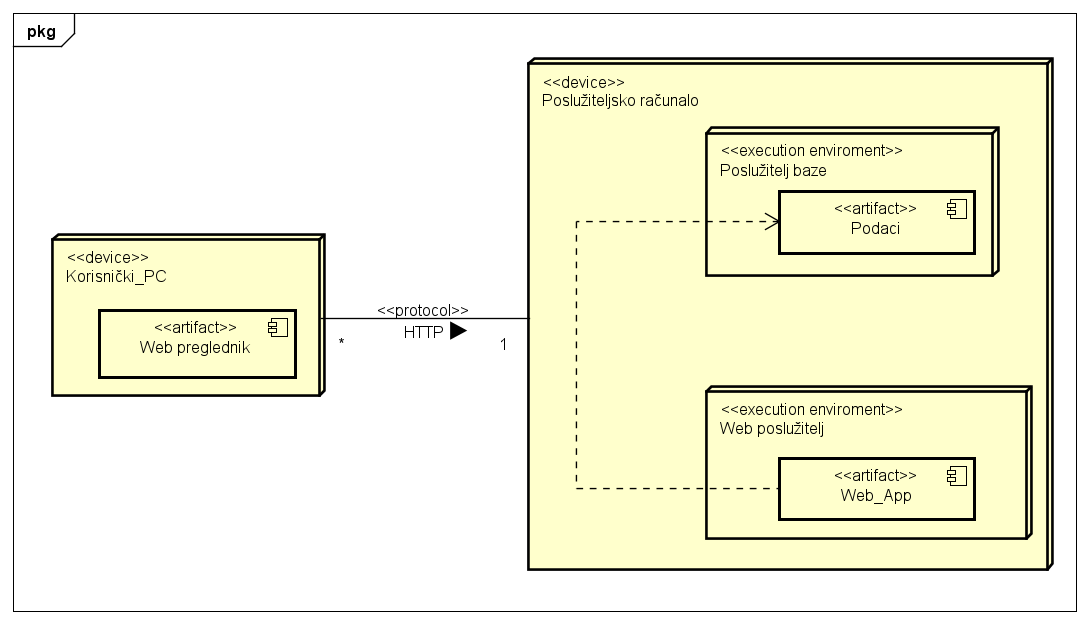
\includegraphics[width=16cm]{slike/Dijagram_razmjestaja.png}
                    \caption{Dijagram razmještaja}
                    \label{fig:DR_01}
                \end{figure}
			    
			\eject 
			
		
		\section{Upute za puštanje u pogon}
		
			\textbf{\textit{dio 2. revizije}}\\
		
			 \textit{U ovom poglavlju potrebno je dati upute za puštanje u pogon (engl. deployment) ostvarene aplikacije. Na primjer, za web aplikacije, opisati postupak kojim se od izvornog kôda dolazi do potpuno postavljene baze podataka i poslužitelja koji odgovara na upite korisnika. Za mobilnu aplikaciju, postupak kojim se aplikacija izgradi, te postavi na neku od trgovina. Za stolnu (engl. desktop) aplikaciju, postupak kojim se aplikacija instalira na računalo. Ukoliko mobilne i stolne aplikacije komuniciraju s poslužiteljem i/ili bazom podataka, opisati i postupak njihovog postavljanja. Pri izradi uputa preporučuje se \textbf{naglasiti korake instalacije uporabom natuknica} te koristiti što je više moguće \textbf{slike ekrana} (engl. screenshots) kako bi upute bile jasne i jednostavne za slijediti.}
			
			
			 \textit{Dovršenu aplikaciju potrebno je pokrenuti na javno dostupnom poslužitelju. Studentima se preporuča korištenje neke od sljedećih besplatnih usluga: \href{https://aws.amazon.com/}{Amazon AWS}, \href{https://azure.microsoft.com/en-us/}{Microsoft Azure} ili \href{https://www.heroku.com/}{Heroku}. Mobilne aplikacije trebaju biti objavljene na F-Droid, Google Play ili Amazon App trgovini.}
			
			
			\eject 

	\chapter{Zaključak i budući rad\hfill}
		
		Zadatak naše grupe bio je razvoj web aplikacije za iznajmljivanje vozila preko interneta (rent a car aplikacija) uz mogućnost upravljanja vozilima, poslovnicama, rezervacijama i recenzijama. Aplikacija na kojoj je radio tim od sedam članova u potpunosti je dovršena nakon petnaest tjedana naporna rada. Provedba projekta odvijala se u dvjema fazama. Radi se o fazi ostvarivanja osnovnih funkcionalnosti web aplikacije, te fazi ostvarivanja različitih implementacijskih detalja. 
		
		\setlength\parindent{24pt}
         Prva faza projekta uključivala je okupljanje tima za razvoj aplikacije, odabir projektnog zadatka, te definiranje ciljeva koje smo kasnije ostvarili. Značajan dio vremena u prvoj fazi zahtijevala je izrada dokumentacije. Kvalitetna dokumentacija nam je uvelike olakšala daljni rad pri realizaciji osmišljenog sustava. Detaljno opisani obrasci uporabe, kao i dijagrami obrazaca uporabe, oslikavajući sve bitne funkcionalnosti, predstavljali su bitan faktor pri izradi aplikacije. Opisivanje modela baze podataka  nam je poslužilo za izradu seed.js dokumenta kojim smo napunili praznu bazu autos, kao i za ostvarenje korištenih razreda. Osim dokumentacije, prvi dio projekta uključivao je i izradu osnovnih funkcionalnosti kao što su registracija, prijava i stvaranje baze podataka.
         
         \setlength\parindent{24pt}
        Druga faza projekta bila je puno intenzivnija nego prva što se tiče samostalnog rada. Uključivala je pisanje programskog koda i manjim dijelom pisanje dokumentacije. Dokumentacija je uključivala izradu UML dijagrama. Neki članovi tima na početku snalazili su se bolje od ostalih pri pisanju programskog koda pa su pomagali ostalim članovima tima. Uz njhovu pomoć svi članovi postali su sposobnima samostalno odraditi svoje zadatke. Manjak iskustva izrade aplikacija za web je predstavljao prepreku pri ostvarivanju dogovorenih ciljeva, no s vremenom svi su se snalazili pri pisanju koda. 
        
        \setlength\parindent{24pt}
        Komunikacija među članovima grupe bila je ostvarena putem Whatsappa čime smo postigli informiranost o napretku projekta, kao i dogovore o mogućim idejama i sastajanjima. Sastanci su bili održani preko platforme Microsoft Teams ili uživo. 
        
        \setlength\parindent{24pt}
        Sudjelovanje na ovakvom projektu bilo je vrijedno iskustvo svim članovima tima. Ovo je naš prvi ovakav projekt. Znanje koje nam je bilo potrebno za ovaj projekt smo jednim dijelom stekli na predmetu Razvoj programske potpore za web i pokretne uređaje, te smo to znanje unaprijedili kroz ovaj projekt uz pomoć interneta i samog iskustva. Iako smo sasvim zadovoljni postignutim uspjehom, uvijek ima mjesta za napredak. 
		
		\eject 
	\chapter*{Popis literature}
		\addcontentsline{toc}{chapter}{Popis literature}
	 	
 		\textbf{\textit{Kontinuirano osvježavanje}}
	
		\textit{Popisati sve reference i literaturu koja je pomogla pri ostvarivanju projekta.}
		
		
		\begin{enumerate}
			
			
			\item  Programsko inženjerstvo, FER ZEMRIS, \url{http://www.fer.hr/predmet/proinz}
			
			\item  I. Sommerville, "Software engineering", 8th ed, Addison Wesley, 2007.
			
			\item  T.C.Lethbridge, R.Langaniere, "Object-Oriented Software Engineering", 2nd ed. McGraw-Hill, 2005.
			
			\item  I. Marsic, Software engineering book``, Department of Electrical and Computer Engineering, Rutgers University, \url{http://www.ece.rutgers.edu/~marsic/books/SE}
			
			\item  The Unified Modeling Language, \url{https://www.uml-diagrams.org/}
			
			\item  Astah Community, \url{http://astah.net/editions/uml-new}
		\end{enumerate}
		
		 
	
	
	\begingroup
	\renewcommand*\listfigurename{Indeks slika i dijagrama}
	%\renewcommand*\listtablename{Indeks tablica}
	%\let\clearpage\relax
	\listoffigures
	%\vspace{10mm}
	%\listoftables
	\endgroup
	\addcontentsline{toc}{chapter}{Indeks slika i dijagrama}


	
	\eject 
		
	\chapter*{Dodatak: Prikaz aktivnosti grupe}
		\addcontentsline{toc}{chapter}{Dodatak: Prikaz aktivnosti grupe}
		
		\section*{Dnevnik sastajanja}
		
		\textbf{\textit{Kontinuirano osvježavanje}}\\
		
		 \textit{U ovom dijelu redovito osvježavamo dnevnik sastajanja prema predlošku.}
		
		\begin{packed_enum}
			\item  sastanak
			
			\item[] \begin{packed_item}
				\item Datum: 6. listopada 2020.
				\item Prisustvovali: Hrvatić, Smolić - Ročak, Blaić, Damjanović, Sekula, Ratko, Huđin
				\item Teme sastanka:
				\begin{packed_item}
					\item  raspodjela rada
					\item  dogovor o korištenju tehnologija
				\end{packed_item}
			\end{packed_item}
			
			%
			
		\end{packed_enum}
		
		\eject
		\section*{Tablica aktivnosti}
		
			\textbf{\textit{Kontinuirano osvježavanje}}\\
			
			 \textit{Napomena: Doprinose u aktivnostima treba navesti u satima po članovima grupe po aktivnosti.}
					
						
			
			\begin{longtabu} to \textwidth {|X[7, l]|X[1, c]|X[1, c]|X[1, c]|X[1, c]|X[1, c]|X[1, c]|X[1, c]|}
								
				\cline{2-8} \multicolumn{1}{c|}{\textbf{}} &     \multicolumn{1}{c|}{\rotatebox{90}{\textbf{Hrvatić Josip }}} & \multicolumn{1}{c|}{\rotatebox{90}{\textbf{Smolić - Ročak Magda }}} &	\multicolumn{1}{c|}{\rotatebox{90}{\textbf{Blaić Krešo }}} &	\multicolumn{1}{c|}{\rotatebox{90}{\textbf{Damjanović Antonio }}} &
				\multicolumn{1}{c|}{\rotatebox{90}{\textbf{Ratko Tomo }}} &
				\multicolumn{1}{c|}{\rotatebox{90}{\textbf{Sekula Dominik }}} &	\multicolumn{1}{c|}{\rotatebox{90}{\textbf{Huđin Matija }}} \\ \hline 
				\endfirsthead
				
			
				\cline{2-8} \multicolumn{1}{c|}{\textbf{}} &     \multicolumn{1}{c|}{\rotatebox{90}{\textbf{Hrvatić Josip}}} & \multicolumn{1}{c|}{\rotatebox{90}{\textbf{Smolić - Ročak Magda }}} &	\multicolumn{1}{c|}{\rotatebox{90}{\textbf{Blaić Krešo }}} &
				\multicolumn{1}{c|}{\rotatebox{90}{\textbf{Damjanović Antonio }}} &	\multicolumn{1}{c|}{\rotatebox{90}{\textbf{Ratko Tomo }}} &
				\multicolumn{1}{c|}{\rotatebox{90}{\textbf{Sekula Dominik }}} &	\multicolumn{1}{c|}{\rotatebox{90}{\textbf{Huđin Matija }}} \\ \hline 
				\endhead
				
				
				\endfoot
							
				 
				\endlastfoot
				
				Upravljanje projektom 		& 7 &  &  &  &  &  & \\ \hline
				Opis projektnog zadatka 	&  &  &  &  &  &  & \\ \hline
				
				Funkcionalni zahtjevi       &  & 0.5 &  &  & 3 & 2 &  \\ \hline
				Opis pojedinih obrazaca 	&  &  &  &  5  &  &  &  \\ \hline
				Dijagram obrazaca 			&  1  &  2  &  2  &  &  &  2  &\\ \hline
				Sekvencijski dijagrami 		&  &  &  &  &  &  &  \\ \hline
				Opis ostalih zahtjeva 		&  &  &  &  & 1 & 1 &  \\ \hline

				Arhitektura i dizajn sustava	 &  &  &  &  &  &  &  \\ \hline
				Baza podataka				&  &  &  &  &  &  &   \\ \hline
				Dijagram razreda 			&  &  &  &  &  &  &   \\ \hline
				Dijagram stanja				&  &  &  &  &  &  &  \\ \hline
				Dijagram aktivnosti 		&  &  &  &  &  &  &  \\ \hline
				Dijagram komponenti			&  &  &  &  &  &  &  \\ \hline
				Korištene tehnologije i alati 		&  &  &  &  &  &  &  \\ \hline
				Ispitivanje programskog rješenja 	&  &  &  &  &  &  &  \\ \hline
				Dijagram razmještaja			&  &  &  &  &  &  &  \\ \hline
				Upute za puštanje u pogon 		&  &  &  &  &  &  &  \\ \hline 
				Dnevnik sastajanja 			&  &  &  &  &  &  &  \\ \hline
				Zaključak i budući rad 		&  &  &  &  &  &  &  \\  \hline
				Popis literature 			&  &  &  &  &  &  &  \\  \hline
				&  &  &  &  &  &  &  \\ \hline \hline
				\textit{Dodatne stavke kako ste podijelili izradu aplikacije} 			&  &  &  &  &  &  &  \\ \hline
				\textit{npr. izrada početne stranice} 				&  &  &  &  &  &  &  \\ \hline 
				\textit{izrada baze podataka} 		 			&  &  &  &  &  &  & \\ \hline 
				\textit{spajanje s bazom podataka} 							&  &  &  &  &  &  &  \\ \hline
				\textit{back end} 							&  &  &  &  &  &  &  \\  \hline
				 							&  &  &  &  &  &  &\\  \hline
				
				
			\end{longtabu}
					
					
		\eject
		\section*{Dijagrami pregleda promjena}
		
		\textbf{\textit{dio 2. revizije}}\\
		
		\textit{Prenijeti dijagram pregleda promjena nad datotekama projekta. Potrebno je na kraju projekta generirane grafove s gitlaba prenijeti u ovo poglavlje dokumentacije. Dijagrami za vlastiti projekt se mogu preuzeti s gitlab.com stranice, u izborniku Repository, pritiskom na stavku Contributors.}
		
	


\end{document} %naredbe i tekst nakon ove naredbe ne ulaze u izgrađen dokument 


